\documentclass[UTF8]{ctexart}
\usepackage[a4paper,margin=2.2cm]{geometry}
\usepackage{booktabs}
\usepackage{graphicx}
\usepackage{float}
\usepackage{xcolor}
\usepackage{listings}
\usepackage{caption}
\usepackage{hyperref}
\hypersetup{colorlinks=true,linkcolor=blue,urlcolor=blue}

\lstdefinestyle{pythoncode}{
  language=Python,
  basicstyle=\ttfamily\scriptsize,
  keywordstyle=\color{blue!70!black},
  commentstyle=\color{green!40!black},
  stringstyle=\color{red!50!black},
  numbers=left,
  numberstyle=\tiny\color{gray},
  stepnumber=1,
  numbersep=6pt,
  frame=single,
  breaklines=true,
  showstringspaces=false,
  tabsize=4
}
\lstset{style=pythoncode}

\title{深度学习课程实验讲稿}
\author{}
\date{}

\begin{document}
\maketitle

\section*{开场}
各位老师同学好，我这次实验一共分为三个部分：第一部分是只用 NumPy 手写 MLP，第二部分是用 PyTorch 实现 CNN 识别 MNIST，第三部分是用 PyTorch 实现 ResNet 并在 MNIST 上训练。

这三个实验不是孤立的，而是从底层到高层逐步递进。第一个实验强调神经网络最基础的前向传播、损失函数、反向传播和参数更新；第二个实验强调卷积网络如何利用局部感受野和参数共享处理图像；第三个实验强调残差连接为什么能够帮助更深的网络稳定训练。

\section{实验一：NumPy MLP}
\subsection{实验目的}
实验一的目标是不用 PyTorch 的自动求导和神经网络模块，只使用 NumPy 实现一个完整的多层感知机分类器。这个实验的重点不是追求复杂模型，而是证明我理解神经网络最底层的训练过程。

数据集使用的是三分类螺旋数据。每个样本是二维坐标，标签有 3 类。选择这个数据集的原因是它不是线性可分的，三类点呈螺旋形交错分布。线性分类器很难用直线把它们分开，但 MLP 可以通过隐藏层和非线性激活函数学习弯曲的分类边界。

\subsection{代码逻辑}
代码主要在 \texttt{01\_numpy\_mlp/mlp\_numpy.py}。整体流程是：先生成螺旋数据，再划分训练集和测试集，然后标准化，最后进入 MLP 的前向传播、损失计算、反向传播和参数更新。

下面这段代码体现了数据生成逻辑。每一类样本用不同的角度范围生成一条螺旋，再加入噪声，最后统一打乱。

\begin{lstlisting}[caption={实验一：三分类螺旋数据生成}]
def make_spiral_data(samples_per_class=160, num_classes=3, noise=0.2, seed=42):
    rng = np.random.default_rng(seed)
    total = samples_per_class * num_classes
    x = np.zeros((total, 2), dtype=np.float64)
    y = np.zeros(total, dtype=np.int64)

    for class_id in range(num_classes):
        ix = range(class_id * samples_per_class, (class_id + 1) * samples_per_class)
        radius = np.linspace(0.0, 1.0, samples_per_class)
        theta = np.linspace(class_id * 4.0, (class_id + 1) * 4.0, samples_per_class)
        theta += rng.normal(0.0, noise, samples_per_class)
        x[ix] = np.c_[radius * np.sin(theta), radius * np.cos(theta)]
        y[ix] = class_id

    indices = rng.permutation(total)
    return x[indices], y[indices]
\end{lstlisting}

模型是一个单隐藏层 MLP。输入层是 2 维，因为每个样本只有两个坐标；隐藏层宽度可以调；输出层是 3 维，对应三个类别。前向传播顺序是：输入先经过第一层线性变换，然后经过激活函数，再经过第二层线性变换，最后用 Softmax 得到类别概率。

\begin{lstlisting}[caption={实验一：MLP 前向传播}]
def forward(self, x):
    z1 = x @ self.w1 + self.b1
    a1 = self.activate(z1)
    logits = a1 @ self.w2 + self.b2
    probabilities = self.softmax(logits)
    cache = {"x": x, "z1": z1, "a1": a1, "probabilities": probabilities}
    return probabilities, cache
\end{lstlisting}

损失函数使用交叉熵，并加入 L2 正则。交叉熵衡量预测分布和真实标签之间的差距，L2 正则限制权重过大，降低过拟合风险。

\begin{lstlisting}[caption={实验一：交叉熵损失与 L2 正则}]
def cross_entropy_loss(self, probabilities, y_true):
    eps = 1e-12
    clipped = np.clip(probabilities, eps, 1.0 - eps)
    data_loss = -np.sum(y_true * np.log(clipped)) / y_true.shape[0]
    reg_loss = 0.5 * self.l2 * (np.sum(self.w1 * self.w1) + np.sum(self.w2 * self.w2))
    return float(data_loss + reg_loss)
\end{lstlisting}

反向传播从 Softmax 加交叉熵的梯度开始，先计算输出层参数梯度，再把梯度传回隐藏层，乘以激活函数导数，最后得到第一层参数梯度。

\begin{lstlisting}[caption={实验一：反向传播核心}]
def backward(self, cache, y_true):
    x = cache["x"]
    z1 = cache["z1"]
    a1 = cache["a1"]
    probabilities = cache["probabilities"]
    batch_size = x.shape[0]

    d_logits = (probabilities - y_true) / batch_size
    d_w2 = a1.T @ d_logits + self.l2 * self.w2
    d_b2 = d_logits.sum(axis=0, keepdims=True)
    d_a1 = d_logits @ self.w2.T
    d_z1 = d_a1 * self.activation_grad(z1)
    d_w1 = x.T @ d_z1 + self.l2 * self.w1
    d_b1 = d_z1.sum(axis=0, keepdims=True)

    self.apply_gradients({"w1": d_w1, "b1": d_b1, "w2": d_w2, "b2": d_b2})
\end{lstlisting}

参数更新实现了三种优化器：普通 GD、Momentum 和 Adam。GD 是直接沿梯度反方向更新；Momentum 会保留速度项，让更新方向更稳定；Adam 使用一阶矩和二阶矩估计，自适应调整每个参数的更新幅度。

\begin{lstlisting}[caption={实验一：三种优化器的参数更新}]
if self.optimizer == "gd":
    params[name] -= self.learning_rate * grad
elif self.optimizer == "momentum":
    self.velocity[name] = self.momentum * self.velocity[name] - self.learning_rate * grad
    params[name] += self.velocity[name]
else:
    self.first_moment[name] = self.adam_beta1 * self.first_moment[name] + (1.0 - self.adam_beta1) * grad
    self.second_moment[name] = self.adam_beta2 * self.second_moment[name] + (1.0 - self.adam_beta2) * (grad * grad)
    m_hat = self.first_moment[name] / (1.0 - self.adam_beta1**self.step)
    v_hat = self.second_moment[name] / (1.0 - self.adam_beta2**self.step)
    params[name] -= self.learning_rate * m_hat / (np.sqrt(v_hat) + self.adam_eps)
\end{lstlisting}

训练循环整体就是：前向传播、计算损失、反向传播、更新参数、记录训练和测试准确率。

\begin{lstlisting}[caption={实验一：训练循环}]
for epoch in range(1, epochs + 1):
    probabilities, cache = self.forward(x_train)
    loss = self.cross_entropy_loss(probabilities, y_train_one_hot)
    self.backward(cache, y_train_one_hot)

    if epoch == 1 or epoch % log_every == 0 or epoch == epochs:
        history.append(
            TrainingMetrics(
                epoch=epoch,
                loss=loss,
                train_accuracy=self.accuracy(x_train, y_train),
                test_accuracy=self.accuracy(x_test, y_test),
            )
        )
\end{lstlisting}

\subsection{实验结果和图的含义}
实验一基础训练测试准确率是 96.67\%。扩展实验比较了 ReLU、Tanh、Sigmoid 三种激活函数，隐藏层宽度 16、32、64、128，学习率 0.1、0.05、0.01、0.005，以及 GD、Momentum、Adam 三种优化器。排名靠前的配置又做了多随机种子复验。最终最优配置是 ReLU 激活、隐藏层宽度 16、Adam 优化器、学习率 0.01，多随机种子平均测试准确率达到 99.17\%。

\begin{table}[H]
\centering
\caption{MLP 超参数搜索靠前配置}
\begin{tabular}{llllll}
\toprule
激活 & 隐藏层 & 学习率 & 优化器 & 测试准确率 & 标准差 \\
\midrule
relu & 16 & 0.01 & adam & 99.17\% & 0.68\% \\
relu & 64 & 0.1 & momentum & 98.61\% & 0.79\% \\
relu & 16 & 0.05 & adam & 98.61\% & 0.39\% \\
relu & 64 & 0.1 & adam & 98.33\% & 0.68\% \\
relu & 64 & 0.05 & adam & 98.33\% & 0.68\% \\
\bottomrule
\end{tabular}

\end{table}

下面这张图是优化器和学习率对测试准确率的影响。横轴是学习率，纵轴是最佳测试准确率，不同曲线代表不同优化器。可以看到 Adam 在多个学习率下都比较稳定，说明自适应学习率对这个手写 MLP 的收敛帮助明显。

\begin{figure}[H]
\centering
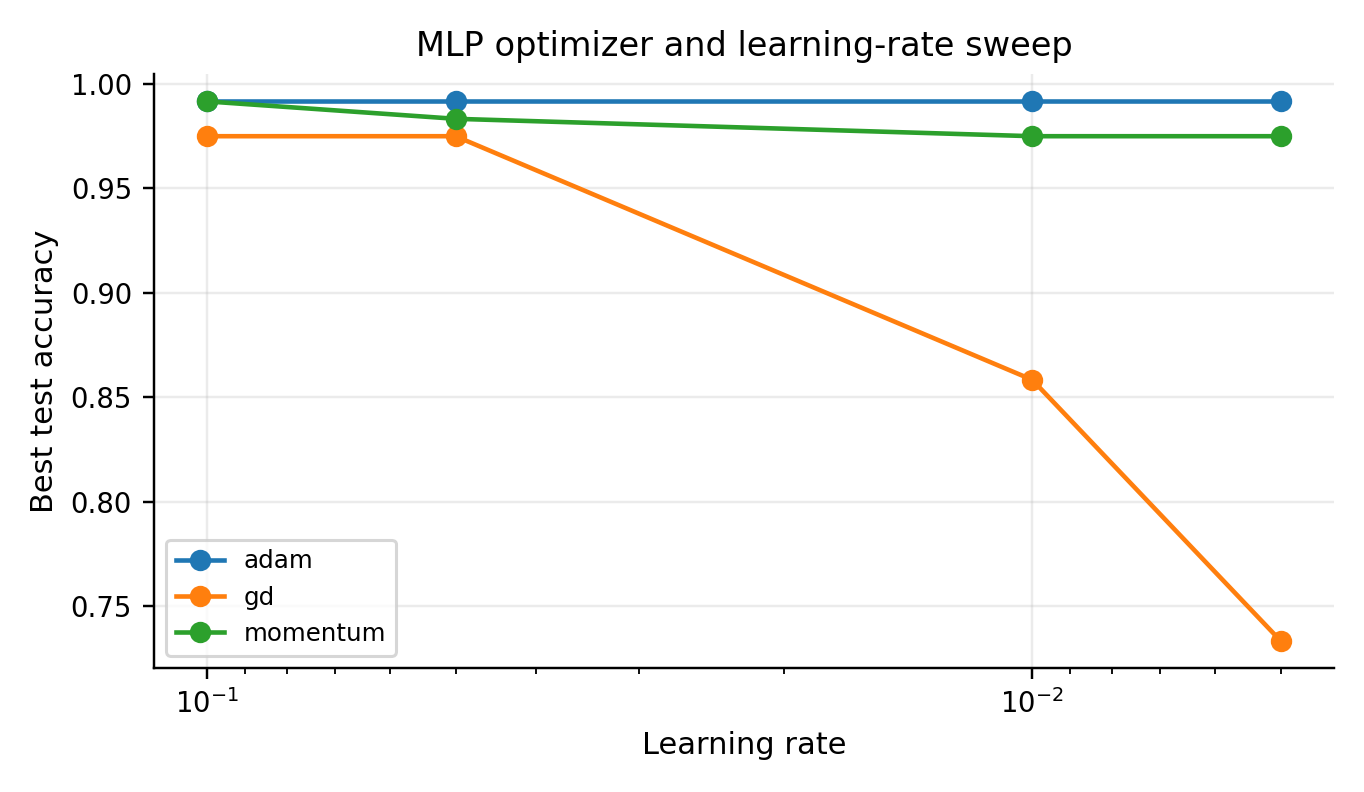
\includegraphics[width=0.78\linewidth]{figures/mlp_optimizer_lr.png}
\caption{MLP 不同优化器与学习率下的最佳测试准确率}
\end{figure}

下面这张图是激活函数和隐藏层宽度的消融。颜色越亮表示测试准确率越高。它说明 ReLU 整体表现比较好，同时隐藏层不是越宽越好。因为这个任务只是二维螺旋分类，隐藏层宽度 16 已经足够表达分类边界。

\begin{figure}[H]
\centering
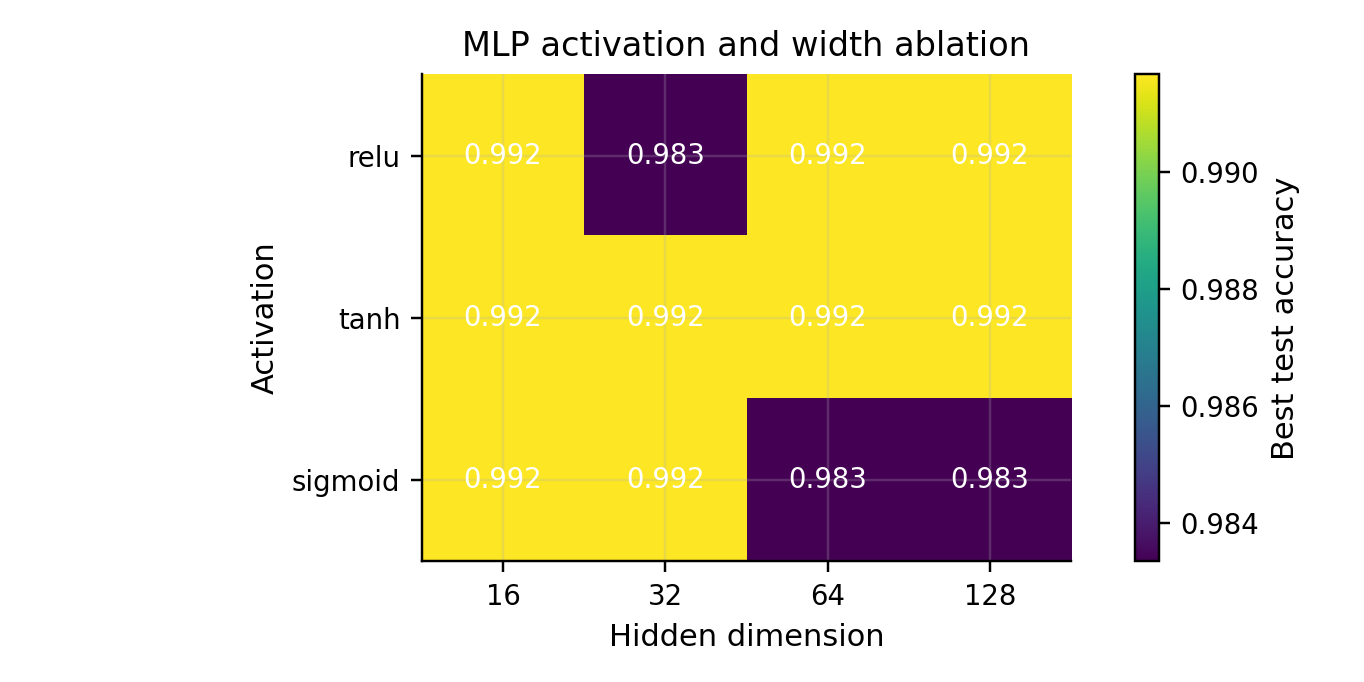
\includegraphics[width=0.78\linewidth]{figures/mlp_activation_hidden.png}
\caption{MLP 激活函数和隐藏层宽度消融}
\end{figure}

下面这张图展示了 MLP 学到的分类边界。背景颜色是模型预测类别，散点是真实数据。可以看到边界是弯曲的，而不是简单直线，这说明隐藏层和非线性激活函数确实学到了螺旋数据的非线性结构。

\begin{figure}[H]
\centering
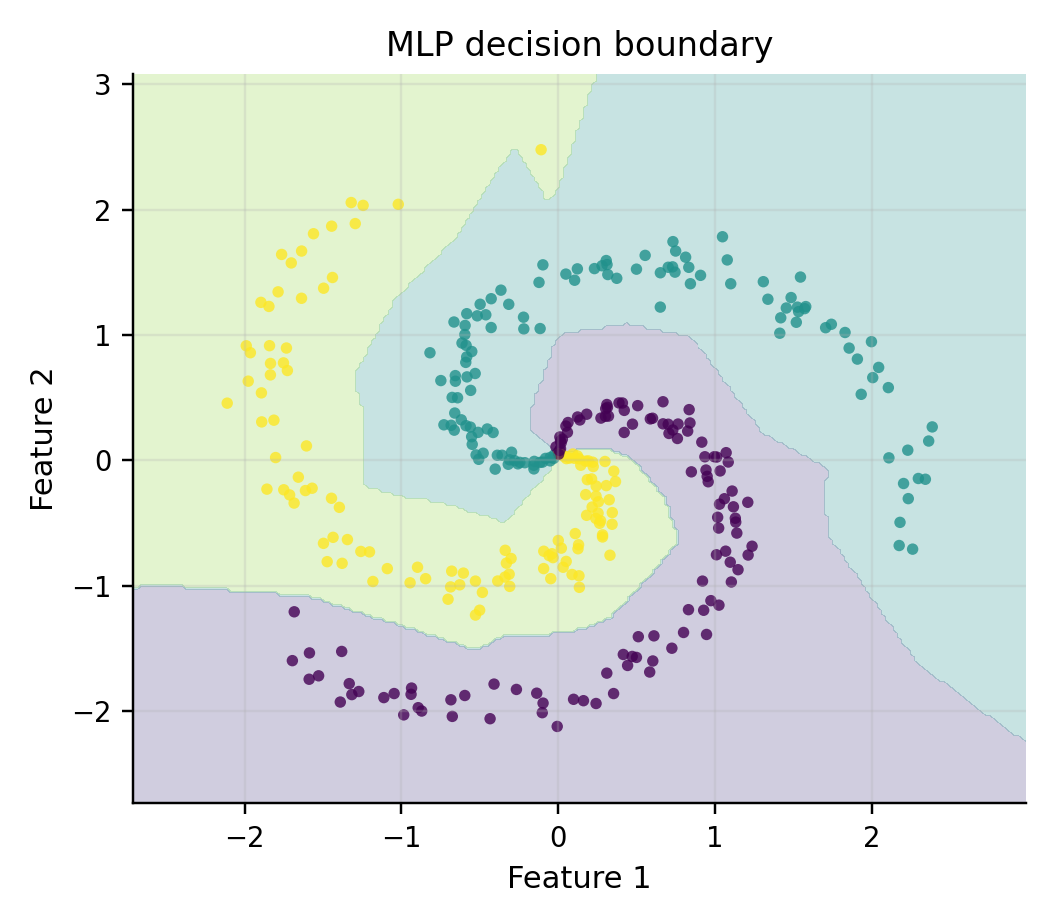
\includegraphics[width=0.62\linewidth]{figures/mlp_decision_boundary.png}
\caption{MLP 在螺旋数据集上的分类边界示例}
\end{figure}

\section{实验二：MNIST CNN}
\subsection{实验目的}
实验二使用 PyTorch 搭建卷积神经网络，对 MNIST 手写数字进行 10 分类。和实验一不同，这里不再手写梯度，而是重点观察 CNN 的结构设计如何影响图像分类效果。

\subsection{代码逻辑}
实验二的基础训练文件是 \texttt{02\_mnist\_cnn/train\_cnn.py}。模型叫 \texttt{SimpleCNN}，由两组卷积块和一个全连接分类器组成。卷积块负责提取局部笔画特征，比如边缘、弯曲和数字局部结构；分类器把卷积特征转换成 10 个类别输出。

\begin{lstlisting}[caption={实验二：CNN 模型结构}]
def conv_block(in_channels, out_channels):
    layers = [
        nn.Conv2d(in_channels, out_channels, kernel_size=kernel_size, padding=padding),
    ]
    if batch_norm:
        layers.append(nn.BatchNorm2d(out_channels))
    layers.append(nn.ReLU())
    if pooling:
        layers.append(nn.MaxPool2d(2))
    return layers

self.features = nn.Sequential(
    *conv_block(1, channels[0]),
    *conv_block(channels[0], channels[1]),
)
self.classifier = nn.Sequential(
    nn.Flatten(),
    nn.Dropout(dropout),
    nn.Linear(feature_dim, 128),
    nn.ReLU(),
    nn.Dropout(dropout),
    nn.Linear(128, 10),
)
\end{lstlisting}

数据加载使用 torchvision 自带的 MNIST。图片先转成 Tensor，再按 MNIST 的均值和标准差归一化。训练集打乱，测试集不打乱。

\begin{lstlisting}[caption={实验二：MNIST 数据加载}]
transform = transforms.Compose(
    [
        transforms.ToTensor(),
        transforms.Normalize((0.1307,), (0.3081,)),
    ]
)
train_dataset = datasets.MNIST(root=data_dir, train=True, download=True, transform=transform)
test_dataset = datasets.MNIST(root=data_dir, train=False, download=True, transform=transform)

train_loader = DataLoader(train_dataset, batch_size=batch_size, shuffle=True, num_workers=num_workers)
test_loader = DataLoader(test_dataset, batch_size=batch_size, shuffle=False, num_workers=num_workers)
\end{lstlisting}

训练流程是标准 PyTorch 分类流程：前向计算 logits，交叉熵计算损失，调用 \texttt{loss.backward()} 自动反向传播，然后优化器更新参数。评估时关闭梯度，只计算平均损失和准确率。

\begin{lstlisting}[caption={实验二：训练一个 epoch}]
for images, labels in loader:
    images = images.to(device)
    labels = labels.to(device)

    optimizer.zero_grad(set_to_none=True)
    logits = model(images)
    loss = criterion(logits, labels)
    loss.backward()
    optimizer.step()

    total_loss += loss.item() * labels.size(0)
    correct += (logits.argmax(dim=1) == labels).sum().item()
    total += labels.size(0)
\end{lstlisting}

实验二有两组扩展实验。第一组固定 CNN 结构，只比较 Adam、SGD、RMSprop 和不同学习率；第二组固定优化策略，比较卷积核大小、通道宽度、BatchNorm、Dropout 和池化。

\subsection{实验结果和图的含义}
基础 CNN 测试准确率为 99.00\%。优化器和学习率搜索中，RMSprop 加 0.0001 的测试准确率最高，为 98.96\%；Adam 加 0.001 的结果也很接近。架构消融中，5x5 卷积核、32/64 通道、BatchNorm、Dropout 等于 0.25 并保留池化的配置最好，测试准确率达到 99.15\%。

\begin{table}[H]
\centering
\caption{CNN 优化器与学习率搜索 Top 配置}
\begin{tabular}{lllll}
\toprule
优化器 & 学习率 & 训练准确率 & 测试准确率 & 测试损失 \\
\midrule
rmsprop & 0.0001 & 98.42\% & 98.96\% & 0.0332 \\
adam & 0.001 & 98.42\% & 98.94\% & 0.0305 \\
adam & 0.0005 & 98.34\% & 98.88\% & 0.0329 \\
rmsprop & 0.0005 & 97.51\% & 98.88\% & 0.0353 \\
rmsprop & 0.001 & 97.31\% & 98.74\% & 0.0381 \\
sgd & 0.01 & 98.19\% & 98.64\% & 0.0408 \\
\bottomrule
\end{tabular}

\end{table}

\begin{table}[H]
\centering
\caption{CNN 架构消融 Top 配置}
\begin{tabular}{lllll}
\toprule
配置 & 消融因素 & 参数量 & 测试准确率 & 测试损失 \\
\midrule
kernel5\_c32-64\_bn\_do25\_pool & kernel\_size & 455114 & 99.15\% & 0.0253 \\
wide\_k3\_c64-128\_bn\_do25\_pool & channels & 879114 & 99.07\% & 0.0289 \\
baseline\_k3\_c32-64\_bn\_do25\_pool & baseline & 421834 & 98.96\% & 0.0298 \\
no\_batch\_norm\_k3\_c32-64\_do25\_pool & batch\_norm & 421642 & 98.95\% & 0.0320 \\
dropout50\_k3\_c32-64\_bn\_pool & dropout & 421834 & 98.95\% & 0.0323 \\
dropout0\_k3\_c32-64\_bn\_pool & dropout & 421834 & 98.86\% & 0.0377 \\
narrow\_k3\_c16-32\_bn\_do25\_pool & channels & 207018 & 98.72\% & 0.0370 \\
\bottomrule
\end{tabular}

\end{table}

下面这张图展示了优化器和学习率组合的真实运行结果。这里我改成了排序条形图，每一条就是一组实际跑过的配置，横轴是测试准确率，颜色代表优化器。原来的热力图会出现空白格，是因为 9 组实验并不是完整的 3 乘 5 网格，而是每个优化器只选了 3 个代表性学习率。现在这张图只展示真实运行过的组合，所以更直观。可以看到大部分合理配置都能达到较高准确率，这是因为 MNIST 本身相对简单；但 SGD 对学习率更敏感，学习率过小时收敛较慢。Adam 和 RMSprop 在短训练周期内更容易得到较高准确率。

\begin{figure}[H]
\centering
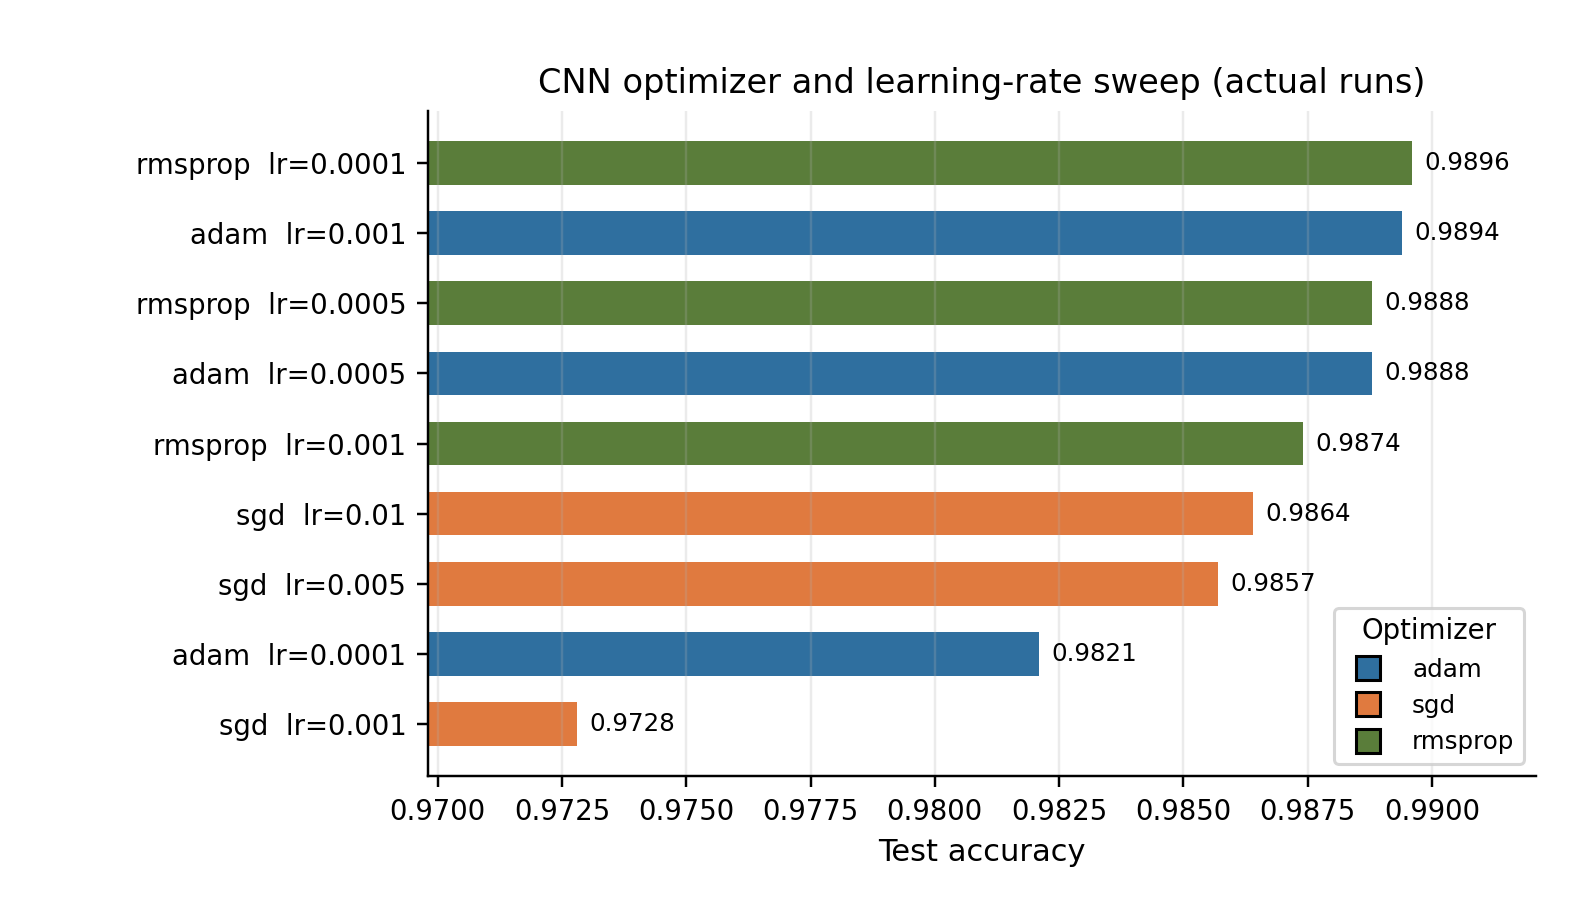
\includegraphics[width=0.78\linewidth]{figures/cnn_optimizer_lr_heatmap.png}
\caption{CNN 优化器与学习率真实运行配置排序图}
\end{figure}

下面这张图是 CNN 架构消融。左侧不再用 C 编号，而是直接写出这一组配置改了什么，比如 5x5 卷积核、加宽通道、去掉 BatchNorm、去掉池化等。右侧的 best 和 lowest 标记分别指出最好和最差的配置。它说明 5x5 卷积核略优，可能是因为 MNIST 的笔画较粗，稍大的感受野可以一次覆盖更多局部形状。无池化配置表现最差，说明池化能降低特征维度，让短周期训练更稳定，也能减少过拟合风险。

\begin{figure}[H]
\centering
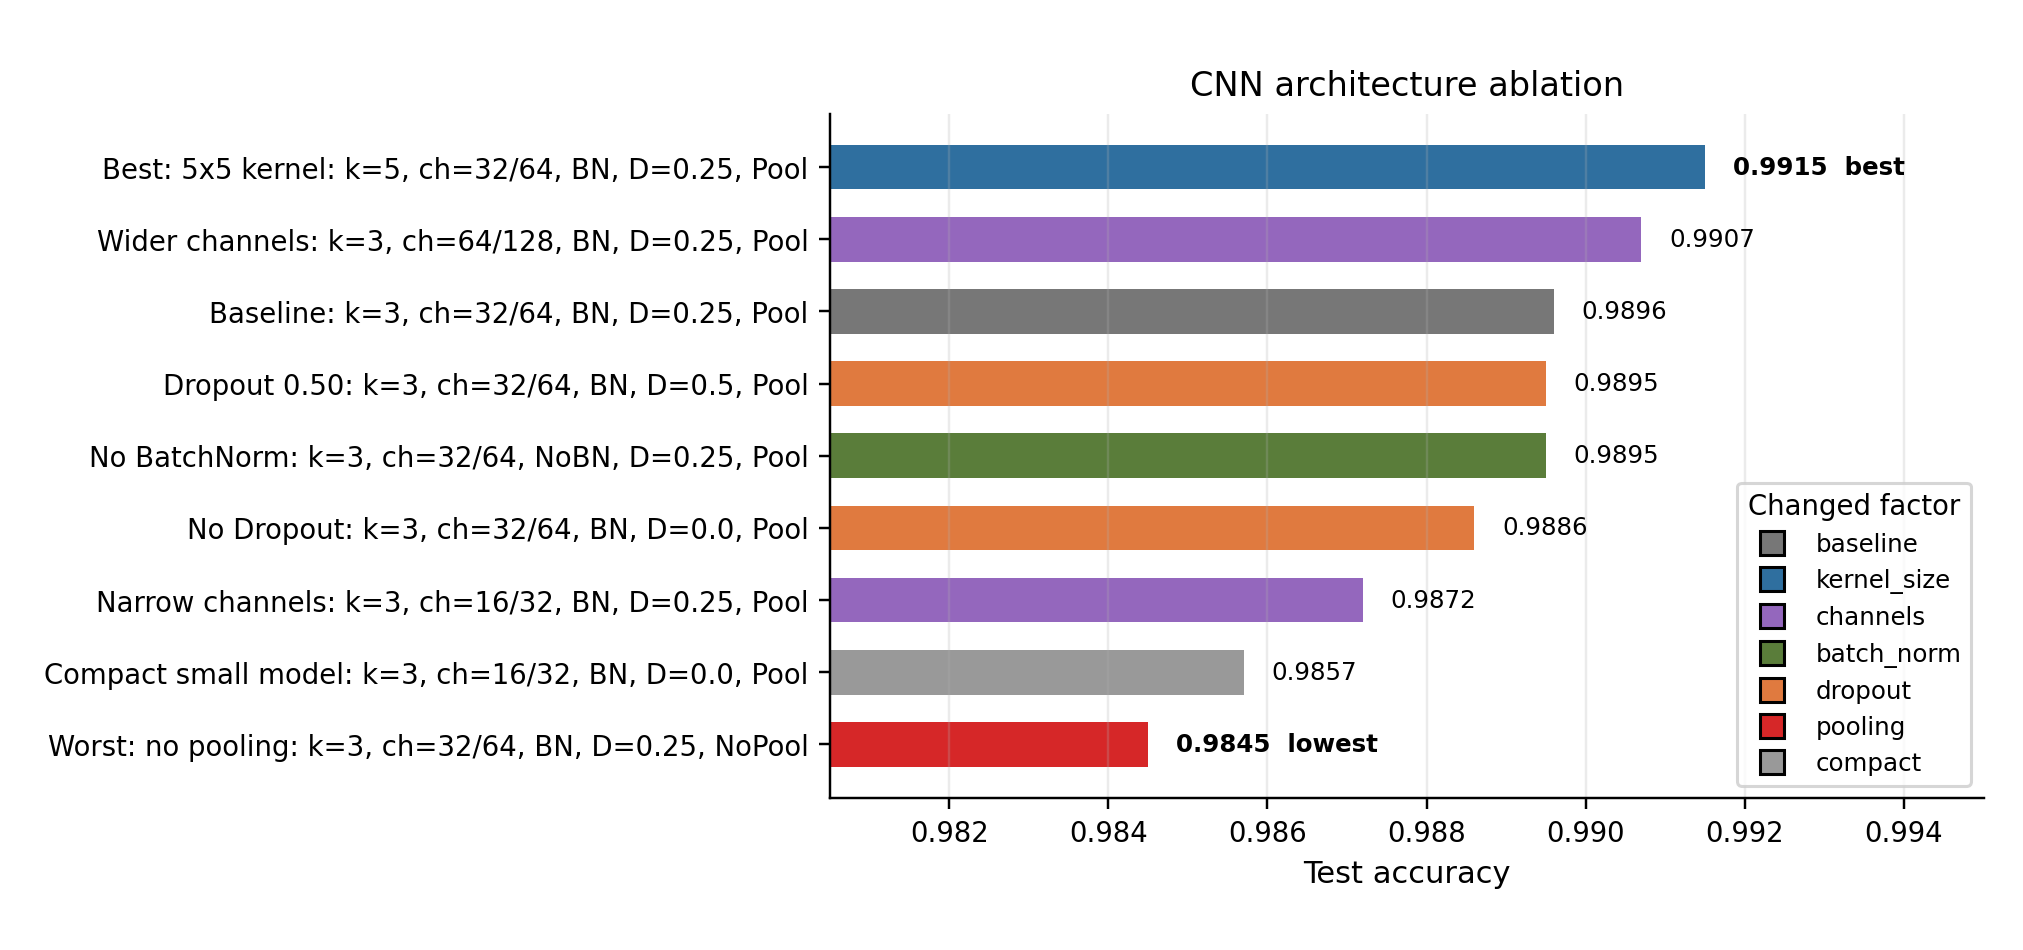
\includegraphics[width=0.92\linewidth]{figures/cnn_arch_ablation.png}
\caption{CNN 架构消融测试准确率，左侧直接标明配置变化}
\end{figure}

\section{实验三：ResNet-MNIST}
\subsection{实验目的}
实验三实现面向 MNIST 的 ResNet。基础要求是 ResNet-50，所以代码里实现了 Bottleneck 模块；同时为了做对比，也实现了 ResNet-18 和 ResNet-34 使用的 BasicBlock。这个实验重点是说明深层网络中残差连接的作用，以及为什么小尺寸 MNIST 图像需要专门适配输入层。

\subsection{代码逻辑}
ResNet 的关键是残差块。BasicBlock 用于 ResNet-18 和 ResNet-34，它由两层 3x3 卷积组成。如果保留残差连接，就把输入 identity 加回输出。

\begin{lstlisting}[caption={实验三：BasicBlock 残差结构}]
def forward(self, x):
    identity = x

    out = self.relu(self.bn1(self.conv1(x)))
    out = self.bn2(self.conv2(out))

    if self.residual:
        if self.downsample is not None:
            identity = self.downsample(x)
        out += identity

    return self.relu(out)
\end{lstlisting}

Bottleneck 用于 ResNet-50。它先用 1x1 卷积降维，再用 3x3 卷积提取特征，最后用 1x1 卷积升维。这样可以在较深网络中控制计算量。

\begin{lstlisting}[caption={实验三：Bottleneck 残差结构}]
def forward(self, x):
    identity = x

    out = self.relu(self.bn1(self.conv1(x)))
    out = self.relu(self.bn2(self.conv2(out)))
    out = self.bn3(self.conv3(out))

    if self.residual:
        if self.downsample is not None:
            identity = self.downsample(x)
        out += identity
    return self.relu(out)
\end{lstlisting}

MNIST 是 1 通道、28x28 的小图，所以默认使用 MNIST stem，也就是 3x3 卷积、stride 为 1。代码中也保留了 ImageNet 风格 stem，也就是 7x7 卷积加 MaxPool，作为对照。

\begin{lstlisting}[caption={实验三：MNIST stem 与 ImageNet stem}]
if stem_type == "mnist":
    self.stem = nn.Sequential(
        nn.Conv2d(1, 64, kernel_size=3, stride=1, padding=1, bias=False),
        nn.BatchNorm2d(64),
        nn.ReLU(inplace=True),
    )
elif stem_type == "imagenet":
    self.stem = nn.Sequential(
        nn.Conv2d(1, 64, kernel_size=7, stride=2, padding=3, bias=False),
        nn.BatchNorm2d(64),
        nn.ReLU(inplace=True),
        nn.MaxPool2d(kernel_size=3, stride=2, padding=1),
    )
\end{lstlisting}

ResNet 主体由四个阶段组成，通道数逐步增加，空间尺寸逐步降低，最后用全局平均池化和全连接层输出 10 类。

\begin{lstlisting}[caption={实验三：ResNet 整体前向传播}]
def forward(self, x):
    x = self.stem(x)
    x = self.layer1(x)
    x = self.layer2(x)
    x = self.layer3(x)
    x = self.layer4(x)
    x = self.avgpool(x)
    x = torch.flatten(x, 1)
    return self.fc(x)
\end{lstlisting}

通过 \texttt{build\_resnet\_mnist}，代码可以选择 ResNet-18、ResNet-34 或 ResNet-50，也可以关闭 residual 做 Plain 网络对照。

\begin{lstlisting}[caption={实验三：选择 ResNet 深度和残差开关}]
def build_resnet_mnist(variant="resnet50", residual=True, stem_type="mnist"):
    if variant == "resnet18":
        return ResNetMNIST(BasicBlock, [2, 2, 2, 2], residual=residual, stem_type=stem_type)
    if variant == "resnet34":
        return ResNetMNIST(BasicBlock, [3, 4, 6, 3], residual=residual, stem_type=stem_type)
    if variant == "resnet50":
        return ResNetMNIST(Bottleneck, [3, 4, 6, 3], residual=residual, stem_type=stem_type)
\end{lstlisting}

\subsection{实验结果和图的含义}
ResNet-50 基线单独训练的测试准确率是 98.72\%。扩展实验中，ResNet-34 加 MNIST stem、Adam、学习率 0.001 的配置最好，测试准确率达到 99.31\%。ResNet-18 的测试准确率是 99.17\%，也比较高。Plain-18 只有 97.81\%，明显低于带残差连接的 ResNet-18，这说明残差连接确实提升了深层网络训练稳定性。ImageNet stem 的结果是 98.85\%，低于 MNIST stem，说明对 28x28 小图来说，过早强下采样会损失笔画细节。

这里补充说明一下：图里的 Baseline: ResNet-50 是在消融 sweep 里和其他配置一起重跑的 ResNet-50，测试准确率是 98.58\%；而 98.72\% 是基础脚本单独训练的结果。图中使用 sweep 内 baseline，是为了让所有消融对比来自同一张结果表。

\begin{table}[H]
\centering
\caption{ResNet 深度与结构消融结果}
\begin{tabular}{llllll}
\toprule
编号与配置 & 因素 & 参数量 & 优化器 & 学习率 & 测试准确率 \\
\midrule
R1: ResNet-34, MNIST, adam 0.001 & depth & 21280970 & adam & 0.001 & 99.31\% \\
R2: ResNet-18, MNIST, adam 0.001 & depth & 11172810 & adam & 0.001 & 99.17\% \\
R3: ResNet-18, MNIST, sgd 0.01 & optimizer & 11172810 & sgd & 0.01 & 99.16\% \\
R4: ResNet-18, MNIST, rmsprop 0.0001 & optimizer & 11172810 & rmsprop & 0.0001 & 98.94\% \\
R5: ResNet-18, ImageNet, adam 0.001 & stem & 11175370 & adam & 0.001 & 98.85\% \\
R6: ResNet-18, MNIST, adam 0.0005 & learning\_rate & 11172810 & adam & 0.0005 & 98.76\% \\
R7: ResNet-50, MNIST, adam 0.001 & depth & 23519690 & adam & 0.001 & 98.58\% \\
R8: Plain-18, MNIST, adam 0.001 & residual & 11172810 & adam & 0.001 & 97.81\% \\
\bottomrule
\end{tabular}

\end{table}

下面这张图展示不同 ResNet 配置的测试准确率。左侧直接写出模型变化，其中 Baseline: ResNet-50 就是任务书要求的基础版本；其他条目是在这个基础上做深度、stem、优化器、学习率和残差连接对比。可以看到 ResNet-34 最好，Plain-18 最差。这个结果说明，准确率提升不只是来自参数量，而是和残差连接、输入 stem 设计、网络深度都有关系。

\begin{figure}[H]
\centering
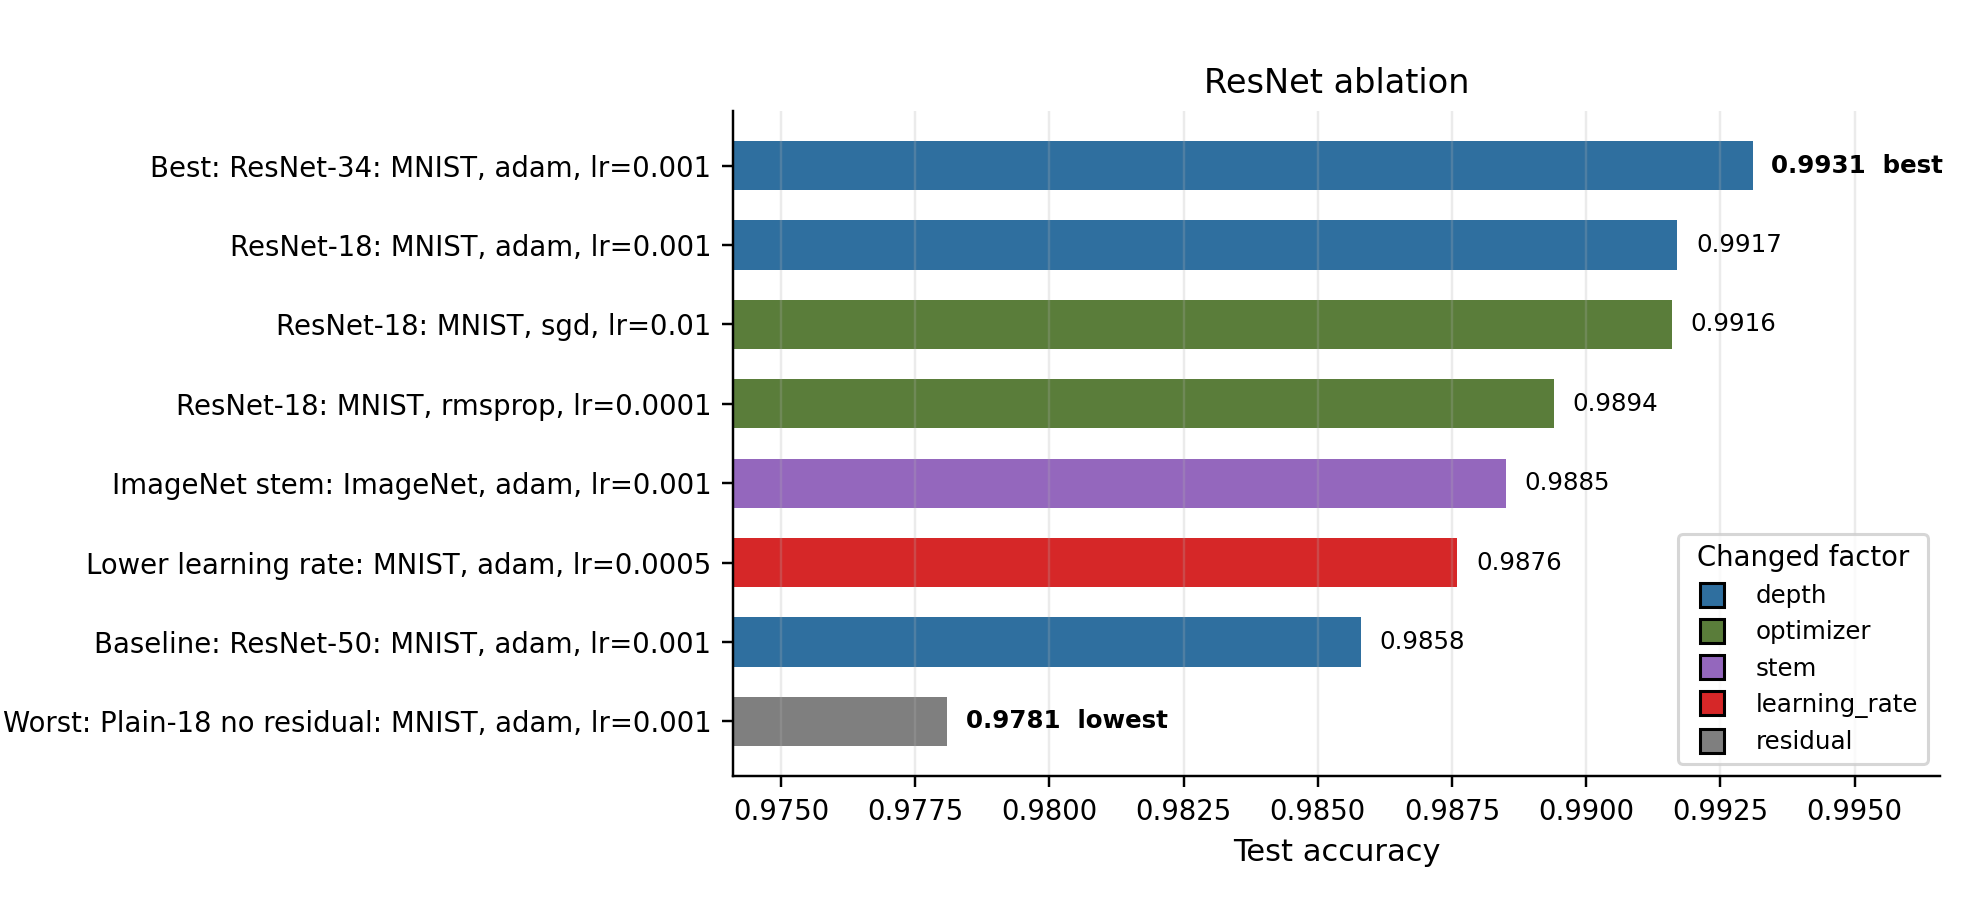
\includegraphics[width=0.92\linewidth]{figures/resnet_ablation.png}
\caption{ResNet 不同配置测试准确率，左侧直接标明模型变化}
\end{figure}

下面这张图展示参数量和测试准确率的关系。每个点旁边直接标明模型含义，比如 Best ResNet-34、Baseline ResNet-50、Plain-18 no residual 等，所以可以直接看出每个点代表哪一个模型。它说明模型参数越多不一定越好。ResNet-50 作为 baseline 参数量比 ResNet-34 更多，但本实验中准确率反而更低。原因是 MNIST 任务比较简单，模型太深不一定带来收益，而且只训练 3 个 epoch 时，更深模型优化成本更高。

\begin{figure}[H]
\centering
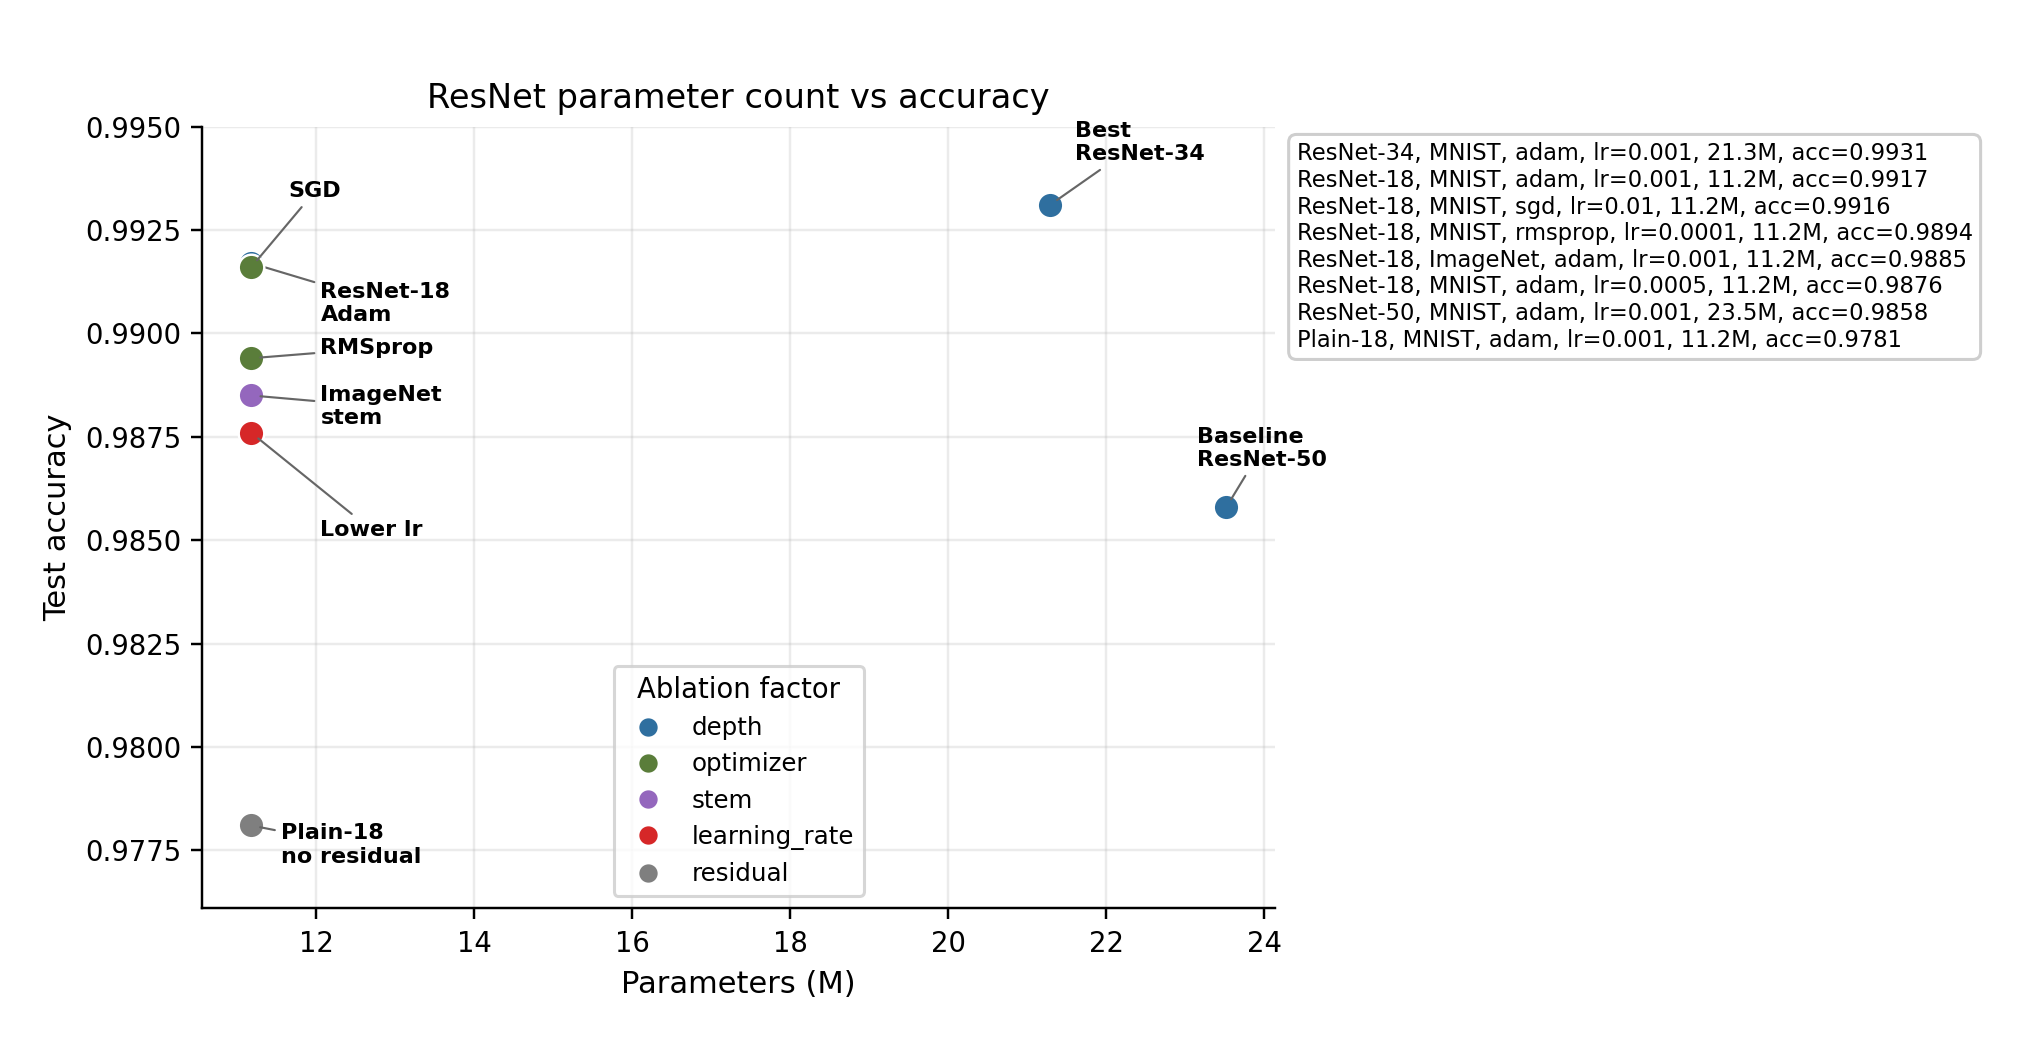
\includegraphics[width=0.84\linewidth]{figures/resnet_params_accuracy.png}
\caption{ResNet 参数量与测试准确率关系，点旁边直接标明模型含义}
\end{figure}

\section*{总结}
最后总结一下，这三个实验分别覆盖了深度学习的三个层次。实验一从零实现 MLP，让我理解神经网络如何完成前向传播、反向传播和参数更新；实验二使用 CNN 处理图像分类，说明卷积、池化、BatchNorm 和 Dropout 对图像识别的作用；实验三实现 ResNet，说明残差连接、网络深度和输入 stem 设计对深层网络训练的影响。

从最终结果看，MLP 最优测试准确率是 99.17\%，CNN 最优测试准确率是 99.15\%，ResNet 最优测试准确率是 99.31\%。三个实验都完成了基础任务，同时通过超参数搜索和结构消融补充了多种情况分析。我的汇报到这里结束，谢谢大家。

\end{document}
